\section{Evaluation}
\label{sec:evaluation}

This section presents the results obtained for evaluating the SOR-Set client
library. The test systems are equipped with Intel Xeon E5520 dual quad core
CPUs with HyperThreading support running at 2.27GHz and with 24GB of RAM,
interconnected through 1Gbps network interfaces. For the datastore, Redis
version 2.6.0-rc6 is used.

The purpose of the first benchmark is to measure how the average time needed to
merge two replicated sets changes as the database size increases. Test
configuration includes 16 Redis instances running on one machine representing
Replica~A, each instance storing one shard of the set. For Replica~B another
machine with identical configuration is used. The client library is deployed
on a third machine. The methodology for measuring is: add 1 million 32-byte
uniform randomly generated elements to Replica~A, measure the time for merging
into Replica~B using a pool of 16 threads, and then repeat the process.

\begin{figure}[t]
  \centering
  \begin{minipage}{1\linewidth}
    \centering
    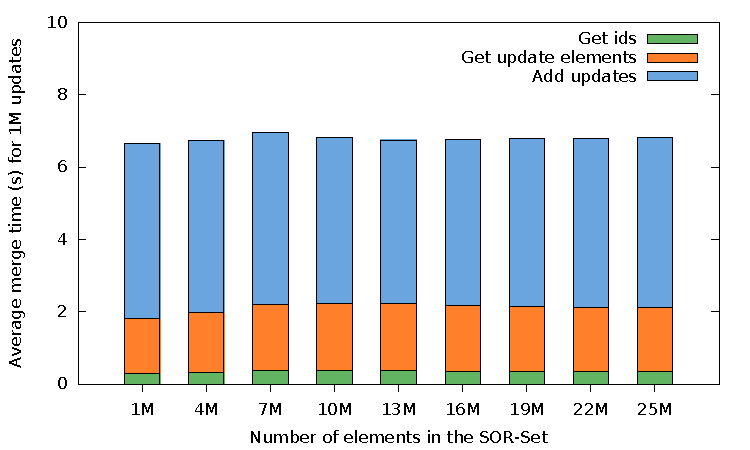
\includegraphics[width=0.9\textwidth]{bench_delta}
    \caption{Delta-based synchronization}
    \label{fig:bench_delta}
  \end{minipage}
\end{figure}

\begin{figure}[t]
  \centering
  \begin{minipage}{1\linewidth}
    \centering
    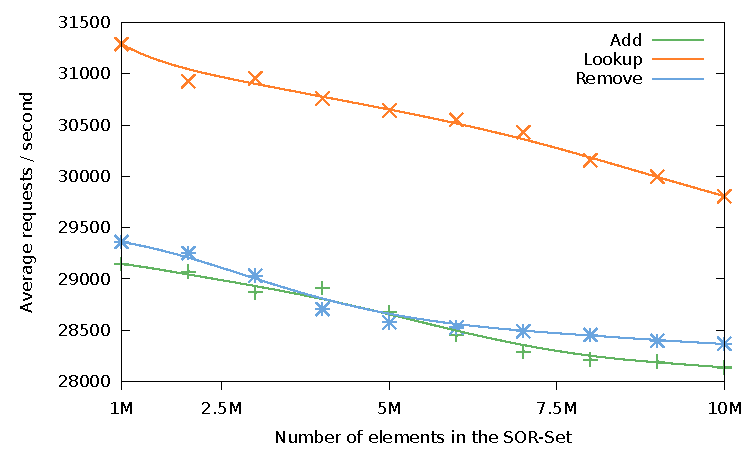
\includegraphics[width=0.9\textwidth]{bench_ops}
    \caption{Throughput for set operations}
    \label{fig:bench_ops}
  \end{minipage}
\end{figure}

Results are presented in Fig.~\ref{fig:bench_delta}. Here are also included
the average timings for each subroutine  of the \textit{merge} procedure
described in Listing~\ref{alg:merge} relevant to these measurements:
getting the element ids, fetching the actual elements from the remote
cluster, and adding the elements to the local cluster. The first observation is
that delta-based synchronization algorithm scales well with the database size.
Since the number of updates between each merge operation is constant, the
timings are also relatively constant. Thus, the \textit{merge} procedure has a
time complexity proportional to the number of updates, i.e. delta size, and not
to the database size. Second, from this plot the average throughput for merging
can be computed to 125,000 update elements per second.

The second benchmark measures the average throughput of all the basic set
operations. For this purpose, a machine with 16 Redis servers acting as a
replica cluster is used. The client library is deployed on another machine to
perform the test: add 1 million 32-byte uniform randomly generated elements to
the set, look them up, remove them, and then repeat the process with more
elements. The drop in throughput in Fig.~\ref{fig:bench_ops} can have one of
two causes: either the operations have time complexity proportional to the
database size, or Redis incurs performance penalty as its database increases.
Listings~\ref{alg:add}, \ref{alg:remove}, and \ref{alg:lookup} show that
only $\mathcal{O}(1)$ Redis operations are used, assuming that same values are
not inserted in the set. This a reasonable assumption since 10 million elements
are generated, each chosen with the same probability from a $2^{8 \times 32}$
space, and thus leading to a low chance of collision. Therefore, updating the
indices is on average a constant operation: \underline{ids}:$e$ contains only
one id and \texttt{lpush} \underline{index}:$rc$:$rs$ is constant. The decline
in performance may be attributed to Redis' management of its internal
structures, such as the global hash table which stores all the keys. As the
database size increases, Redis has to adjust the capacity of this hash, making a
simple \texttt{get} operation on any key costly. This is not visible in
Fig.~\ref{fig:bench_delta} because the timings are dominated there by client
operations.

The reason why a better throughput is obtained for \textit{merge} has two
causes. First, each of \textit{add}, \textit{lookup}, and \textit{remove} is
implemented using Lua scripts for which Redis guarantees to execute in an
atomic way. This is needed to ensure that updating the elements and the indices
in the database does not interleave with other Redis commands. Second, fetching
the elements and distributing the updates in the \textit{merge} procedure are
done using pipelines: sending multiple Redis commands without waiting for a
reply from the server, thus saving the round-trip-time of each request.
Unfortunately, the same technique cannot be used for the other procedures
because both \textit{add} and \textit{remove} increment a counter to generate
the id for each element, while \textit{lookup} must first fetch all ids of one
element. This means we have to wait for a reply from Redis before calling the
subsequent commands, i.e. basic set operations contain synchronous calls to
Redis which make them unsuitable for pipelining. This is not considered to be a
problem since these procedures are independent and are usually issued by
different clients, as opposed to the subroutines of one \textit{merge} call.